% !TeX program = xelatex 

\PassOptionsToPackage{prologue, dvipsnames}{xcolor}
\documentclass[AutoFakeBold,AutoFakeSlant]{beamer}
\usetheme{metropolis}           % Use metropolis theme
\setbeamercovered{transparent}
\usepackage{listings}
\usepackage{ThinctPPT}
 
% 支持中文的设置
\usepackage{xeCJK}
\usepackage{fontspec}
\setCJKmainfont[ItalicFont=思源宋体,BoldFont=SourceHanSerifSC-Bold]{Source Han Serif SC}
\newcommand{\KaiTi}{\CJKfontspec{楷体}}%用命令\fzkaiti调用方正楷体简体

% other packages
\usepackage{latexsym,amsmath,xcolor,multicol,booktabs,calligra}
\usepackage{graphicx,pstricks,listings,stackengine}

\title{\textbf{贪吃蛇}\\反汇编代码分析报告}
\date{\today}
\author{
\includegraphics[width=0.26\linewidth]{ShowMe}\\THINCT}
\begin{document}
\maketitle

\section{SnakeGame}
\subsection{SnakeGame::update}

% Using typewriter font: \ttfamily inside \lstset
\begin{frame}[fragile]
    \LogoFrametitle{EBX 代替当前的函数栈底}
    \begin{x86asmcode}
        004079C0  push  ebx
        004079C1  mov   ebx, esp
        004079C3  sub   esp, 8
        004079C6  and   esp, -8
        004079C9  add   esp, 4
        004079CC  push  ebp
        004079CD  mov   ebp, [ebx+4]
        004079D0  mov   [esp+4], ebp
        004079D4  mov   ebp, esp\end{x86asmcode}
    \begin{enumerate}
        \item 当eip在.text:004079C0处,esp所指向的是ret addr.
        \item 当eip在.text:004079C1处,ebx 所指向的是esp-4.此时:
              \begin{itemize}
                  \item ebx+4指向的是ret addr
                  \item ebx+8 指向的是第一个参数
              \end{itemize}
    \end{enumerate}
\end{frame}


\begin{frame}[fragile]{EBX 代替当前的函数栈底}
    \begin{x86asmcode}
        004079C3  sub   esp, 8
        004079C6  and   esp, 0FFFFFFF8h
        004079C9  add   esp, 4
        004079CC  push  ebp\end{x86asmcode}
    esp实现了向下最近的8的倍数取证。比如12取整就是8,16取整就是16,18取整就是16.因为是针对栈结构地址取整,所以越是往小的方向越安全,因为对于栈结构来讲,越小的地址是没有用过的地址。所以后面的ebp,esp, ebp只能作为局部变量的索引,而对于参数的索引,用ebx比较合适。

    \textbf {总结:}\\
    \emph {对于这个函数来讲,并不是按照套路ebp作为局部变量和函数参数的唯一参考.}
\end{frame}

\begin{frame}[fragile]
    \LogoFrametitle{operator += 传参}
    \begin{x86asmcode}
        004079FF  mov   eax, [ebx+8]
        00407A02  mov   ecx, [eax+4]
        00407A05  push  ecx
        00407A06  mov   edx, [eax]
        00407A08  push  edx
        00407A09  mov   eax, [ebp-2Ch]
        00407A0C  add   eax, 28h ; '('
        00407A0F  push  eax
        00407A10  call  sf::operator+=(sf::Time &,sf::Time)\end{x86asmcode}
    \begin{itemize}
        \item 从0x00407A09到0x00407A0F是第一个参数,已知[ebp-2Ch]为this,所以第一个参数为this->offset28h,并且为sf::Time引用类型.所以\textbf{\textit{sf::Time* this->offset28h}}.
    \end{itemize}
\end{frame}

\begin{frame}[fragile]{operator += 传参}
    \begin{x86asmcode}
        004079FF  mov   eax, [ebx+8]
        00407A02  mov   ecx, [eax+4]
        00407A05  push  ecx
        00407A06  mov   edx, [eax]
        00407A08  push  edx
        00407A09  mov   eax, [ebp-2Ch]
        00407A0C  add   eax, 28h ; '('
        00407A0F  push  eax
        00407A10  call  sf::operator+=(sf::Time &,sf::Time)\end{x86asmcode}
    \begin{itemize}
        \item 0x004079FF已推导出为当前函数的第一个参数,而0x00407A02到0x00407A08是连续的内存,从call得知这个连续的内存是sf::Time类型,所以推导出[ebx+8]是sf::Time*类型,即\textit{\textbf{sf::Time* [ebx+8]}}
    \end{itemize}
\end{frame}

\begin{frame}[fragile]{operator += 传参}
    \textit{\textbf{总结:}} \\
    operator += 第一个参数是传地址,第二个参数是传值,只不过sf::Time的内存是8个字节,所以从起始地址连续压栈2次.本重载函数主要需要掌握的是:\textit{\textbf{不能根据push来判断函数的参数个数}}.
\end{frame}

\begin{frame}[fragile]
    \LogoFrametitle{函数的返回值才是第一个参数}
    \begin{x86asmcode}
        00407A19 mov    ecx, [ebp-2Ch]
        00407A1C movss  xmm0, ds:__real@3f800000
        00407A24 divss  xmm0, dword ptr [ecx+24h]
        00407A29 push   ecx
        00407A2A movss  dword ptr [esp], xmm0
        00407A2F lea    edx, [ebp-28h]
        00407A32 push   edx
        00407A33 call   ds:__imp_?seconds@sf@@YA?AVTime@1@M@Z ; sf::seconds(float) \end{x86asmcode}
    0x00407A2F处压栈的是第一个参数,为局部变量(\textbf{暂存临时返回值}),0x00407A29和0x00407A2A压栈第二个参数,其中push只是占位作用,0x00407A2A才是第二个参数的值,也就是计算出来的浮点数.
\end{frame}

\begin{frame}[fragile]{函数的返回值才是第一个参数}
    \begin{x86asmcode}
        7AC94C90  movss  xmm0,dword ptr [esp+8]
        7AC94C96  mulss  xmm0,dword ptr ds:[7AC982B8h]
        7AC94C9E  call   7AC9600E
        7AC94CA3  mov    ecx,dword ptr [esp+4]
        7AC94CA7  mov    dword ptr [ecx],eax
        7AC94CA9  mov    eax,ecx
        7AC94CAB  mov    dword ptr [ecx+4],edx
        7AC94CAE  ret \end{x86asmcode}
    观察调用的函数,分别从0x7AC94CA3和0x7AC94CA9可知:第一个参数也是该函数的返回值,所以可以推断出:\textbf{函数的返回值才是第一个参数,并且该函数其实只有一个参数},即0x00407A2A处压栈的参数.
\end{frame}


\begin{frame}[fragile]
    \LogoFrametitle{参数与函数可能隔了几个call}
    \begin{x86asmcode}
        00407B1A  push    1 ; includesHead
        00407B1C  mov     ecx, [ebp-2Ch]
        00407B1F  add     ecx, 1408h
        00407B25  call    sf::Transformable::getPosition(void)
        00407B2B  push    eax ; location
        00407B2C  mov     ecx, [ebp-2Ch]
        00407B2F  add     ecx, 30h ; this
        00407B32  call    Snake::collidesWith(sf::Vector2<float> const &,bool)\end{x86asmcode}
    0x00407B1A处压栈参数,在0x00407B25 call之后并没有平栈.通过动态调试得知\textbf{0x00407B25前后esp没有变化,说明该call是没有参数的},跟进0x00407B25 call直接将以地址给eax了,直接说明了\textbf{0x00407B1A push不是0x00407B25 call使用的}.
\end{frame}

\begin{frame}[fragile]{参数与函数可能隔了几个call}
    \begin{x86asmcode}
        00407B1A  push    1 ; includesHead
        00407B1C  mov     ecx, [ebp-2Ch]
        00407B1F  add     ecx, 1408h
        00407B25  call    sf::Transformable::getPosition(void)
        00407B2B  push    eax ; location
        00407B2C  mov     ecx, [ebp-2Ch]
        00407B2F  add     ecx, 30h ; this
        00407B32  call    Snake::collidesWith(sf::Vector2<float> const &,bool)\end{x86asmcode}
    分析0x00407B32 call,得出0x00407B2B是第一个参数,上面的0x00407B1A是第二个参数.    是因为动态调试发现经过0x00407B32 call前后,esp变化为8,所以直接找最近的栈的两个push即可.
\end{frame}

\begin{frame}[fragile]{参数与函数可能隔了几个call}
    \textbf{总结:}
    \begin{enumerate}
        \item 通过动态调试观察esp变化来判断参数的个数
        \item 经过编译器的优化,函数的push可能在其他call之前进行压栈的
    \end{enumerate}
    \textbf{思考:} \\
    在函数被调用前后观察esp的变化,是不是就能确定函数的调用约定了呢?
\end{frame}

\subsection{SnakeGame::update推测this的成员类型}
\begin{frame}[fragile]
    \LogoFrametitle{[ebp-2Ch]存放this,加法偏移识别this的成员变量}
    \tiny
    \linespread{1.2} \selectfont
    \begin{x86asmcode}
        00407A16  add     esp, 0Ch
        00407A19  mov     ecx, [ebp-2Ch]
        00407A1C  movss   xmm0, ds:__real@3f800000
        00407A24  divss   xmm0, dword ptr [ecx+24h] ; float : this->offset24h
        00407A29  push    ecx
        00407A2A  movss   dword ptr [esp], xmm0 ; esp->ecx  [esp]=ds:__real@3f800000
        00407A2F  lea     edx, [ebp-28h] ; sf::seconds的返回值存放的临时变量
        00407A32  push    edx
        00407A33  call    ds:__imp_?seconds@sf@@YA?AVTime@1@M@Z ; sf::seconds(float)

        00407A44  mov     edx, [ebp-2Ch]
        00407A47  mov     eax, [edx+2Ch]
        00407A4A  push    eax
        00407A4B  mov     ecx, [edx+28h] ; sf::Time : this->offset28h
        00407A4E  push    ecx
        00407A4F  call    ds:__imp_??Psf@@YA_NVTime@0@0@Z ; sf::operator>=(sf::Time,sf::Time)
        00407A55  add     esp, 10h

        00407A6A  push    ecx
        00407A6B  mov     edx, [ebp-2Ch]
        00407A6E  add     edx, 28h ; sf::Time : this->offset28h
        00407A71  push    edx
        00407A72  call    ds:__imp_??Zsf@@YAAAVTime@0@AAV10@V10@@Z ; sf::operator-=(sf::Time &,sf::Time)
        00407A78  add     esp, 0Ch\end{x86asmcode}
\end{frame}


\begin{frame}[fragile]{[ebp-2Ch]存放this,加法偏移识别this的成员变量}
    \tiny
    \linespread{0.9} \selectfont
    \begin{x86asmcode}
        00407A90  mov     ecx, [ebp-2Ch]
        00407A93  add     ecx, 13F0h      ; std::deque<Direction> : this->offset13F0h
        00407A99  call    ?front@?$deque@VDirection@@V?$allocator@VDirection@@@std@@@std@@QAEAAVDirection@@XZ ; std::deque<Direction>::front(void)

        00407ACC  push    eax             ; right
        00407ACD  mov     ecx, [ebp-2Ch]
        00407AD0  add     ecx, 1408h
        00407AD6  call    ds:__imp_?getPosition@Transformable@sf@@QBEABV?$Vector2@M@2@XZ ; sf::Transformable::getPosition(void)

            00407AFE  push    edx             ; result
            00407AFF  mov     ecx, [ebp-2Ch]
            00407B02  add     ecx, 4Ch ; BackgroundGrid : this->offset4Ch
            00407B05  call    ?generateRandomPosition@BackgroundGrid@@QAE?AV?$Vector2@M@sf@@XZ ; BackgroundGrid::generateRandomPosition(void)

        00407B0B  mov     ecx, [ebp-2Ch]
        00407B0E  add     ecx, 1408h ; sf::Transformable : this->offset1408h
        00407B14  call    ds:__imp_?setPosition@Transformable@sf@@QAEXABV?$Vector2@M@2@@Z ; sf::Transformable::setPosition(sf::Vector2<float> const &)

        00407C00  mov     ecx, [ebp-2Ch]
        00407C03  add     ecx, 30h ; Snake : this->offset30h
        00407C06  call    ?setColor@Snake@@QAEXVColor@sf@@@Z ; Snake::setColor(sf::Color)

        00407C58  mov     ecx, [ebp-2Ch]
        00407C5B  add     ecx, 30h  ; Snake : this->offset30h
        00407C5E  call    ?length@Snake@@QBEIXZ ; Snake::length(void)\end{x86asmcode}
\end{frame}

\begin{frame}[fragile]{[ebp-2Ch]存放this,加法偏移识别this的成员变量}
    \normalsize
    \linespread{5} \selectfont
    \textbf{总结:} \\
    在同一个函数中,找到this变量,将所有基于该变量偏移的片段截取出来,结合已知的调用函数原型推导变量的含义和类型.
    \linespread{1} \selectfont
\end{frame}


\subsection{SnakeGame::SnakeGame推测this的成员类型}
\begin{frame}[fragile]
    \LogoFrametitle{[ebp-14h]存放this,加法偏移识别this的成员变量}
    \tiny
    \linespread{0.5} \selectfont
    \begin{x86asmcode}
        004074AC mov     [ebp-14h], ecx
        004074C6 mov     edx, [ebp-14h]
        004074C9 mov     dword ptr [edx], offset ??_7SnakeGame@@6B@

        004074D1 mov     ecx, [ebp-14h]
        004074D4 add     ecx, 10h        ; this
        004074D7 call    ??0Direction@@QAE@H@Z ; Direction::Direction(int)

        004074ED mov     ecx, [ebp-14h]
        004074F0 add     ecx, 14h
        004074F3 call    ds:__imp_??0Color@sf@@QAE@EEEE@Z ; sf::Color::Color(uchar,uchar,uchar,uchar)

        0040750D mov     ecx, [ebp-14h]
        00407510 add     ecx, 18h
        00407513 call    ds:__imp_??0Color@sf@@QAE@EEEE@Z ; sf::Color::Color(uchar,uchar,uchar,uchar)

        00407524 mov     ecx, [ebp-14h]
        00407527 add     ecx, 1Ch
        0040752A call    ds:__imp_??0Color@sf@@QAE@EEEE@Z ; sf::Color::Color(uchar,uchar,uchar,uchar)

        0040753B mov     ecx, [ebp-14h]
        0040753E add     ecx, 20h ; ' '
        00407541 call    ds:__imp_??0Color@sf@@QAE@EEEE@Z ; sf::Color::Color(uchar,uchar,uchar,uchar)

        00407547 mov     eax, [ebp-14h]
        0040754A movss   xmm0, ds:__real@41200000
        00407552 movss   dword ptr [eax+24h], xmm0\end{x86asmcode}
\end{frame}

\begin{frame}[fragile]{[ebp-14h]存放this,加法偏移识别this的成员变量}
    \tiny
    \linespread{0.5} \selectfont
    \begin{x86asmcode}
        00407557 mov     ecx, [ebp-14h]
        0040755A add     ecx, 28h ; '('
        0040755D call    ds:__imp_??0Time@sf@@QAE@XZ ; sf::Time::Time(void)

        0040778D mov     ecx, [ebp-14h]
        00407790 add     ecx, 13F0h      ; this
        00407796 call    ??0?$deque@VDirection@@V?$allocator@VDirection@@@std@@@std@@QAE@XZ ; std::deque<Direction>::deque<Direction>(void)

        004077E0 mov     ecx, [ebp-14h]
        004077E3 add     ecx, 1404h
        004077E9 call    ds:__imp_?setFillColor@Shape@sf@@QAEXABVColor@2@@Z ; sf::Shape::setFillColor(sf::Color const &)
        004077EF

        004077F6 mov     ecx, [ebp-14h]
        004077F9 add     ecx, 4Ch ; 'L'  ; this
        004077FC call    ?generateRandomPosition@BackgroundGrid@@QAE?AV?$Vector2@M@sf@@XZ ; BackgroundGrid::generateRandomPosition(void)

            00407811 push    1
            00407813 mov     ecx, [ebp-14h]
            00407816 add     ecx, 1408h
            0040781C call    ds:__imp_?getPosition@Transformable@sf@@QBEABV?$Vector2@M@2@XZ ; sf::Transformable::getPosition(void)

        00407822 push    eax             ; location
        00407823 mov     ecx, [ebp-14h]
        00407826 add     ecx, 30h ; '0'  ; this
        00407829 call    ?collidesWith@Snake@@QBE_NABV?$Vector2@M@sf@@_N@Z ; Snake::collidesWith(sf::Vector2<float> const &,bool)\end{x86asmcode}
\end{frame}


\begin{frame}[fragile]{[ebp-14h]存放this,加法偏移识别this的成员变量}
    \textbf{总结:} \\
    \linespread{1.6} \selectfont
    一般构造函数会对所有成员变量进行初始化的,所以从构造函数来分析this的成员变量是一个不错的选择.
\end{frame}

\begin{frame}[fragile]
    \LogoFrametitle{上面this偏移分析的结构梳理}
    \footnotesize
    \begin{table}[htbp] % 自动找最合适的位置放置该表格
        \centering % 整个表格居中
        \caption{SnakeGame Parse}
        \begin{tabular}{p{1cm}p{5cm}}
            \toprule
            \multicolumn{2}{l}{\textbf{Class members by offset}} \\
            \emph{+10h  } & m\_Direction\_1                      \\
            \emph{+14h  } & m\_sf\_\_Time\_1                     \\
            \emph{+18h  } & m\_sf\_\_Color\_1                    \\
            \emph{+1Ch  } & m\_sf\_\_Color\_2                    \\
            \emph{+20h  } & m\_sf\_\_Color\_3                    \\
            \emph{+24h  } & m\_float\_second\_1                  \\
            \emph{+28h  } & m\_sf\_\_Time\_2                     \\
            \emph{+30h  } & m\_object\_Snake\_1                  \\
            \emph{+4Ch  } & m\_BackgroundGrid                    \\
            \emph{+13F0h} & m\_std\_\_deque\_Direction\_1        \\
            \emph{+1404h} & m\_sf\_\_Shape                       \\
            \emph{+1408h} & m\_sf\_\_Transformable\_position     \\
            \bottomrule
        \end{tabular}
    \end{table}
\end{frame}


\subsection{SnakeGame CE动态监视this的成员类型}
\begin{frame}[fragile]
    \LogoFrametitle{CE 平坦式内存}
    \begin{figure}
        \centering % 将整个 figure 居中
        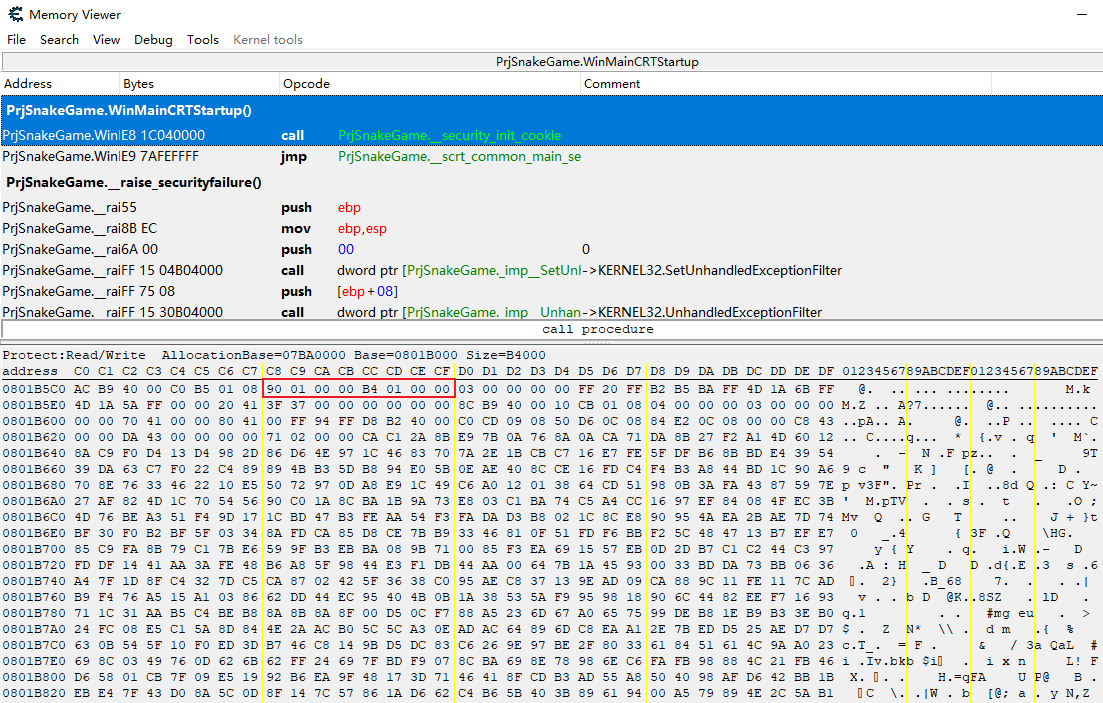
\includegraphics[width=\linewidth]{CE_MEM_FLAT.png}
        \caption{平坦式内存}
        \label{fig:CE_MEM_FLAT}
    \end{figure}
\end{frame}


\begin{frame}[fragile]
    \LogoFrametitle{CE 层级内存}
    \begin{figure}
        \centering % 将整个 figure 居中
        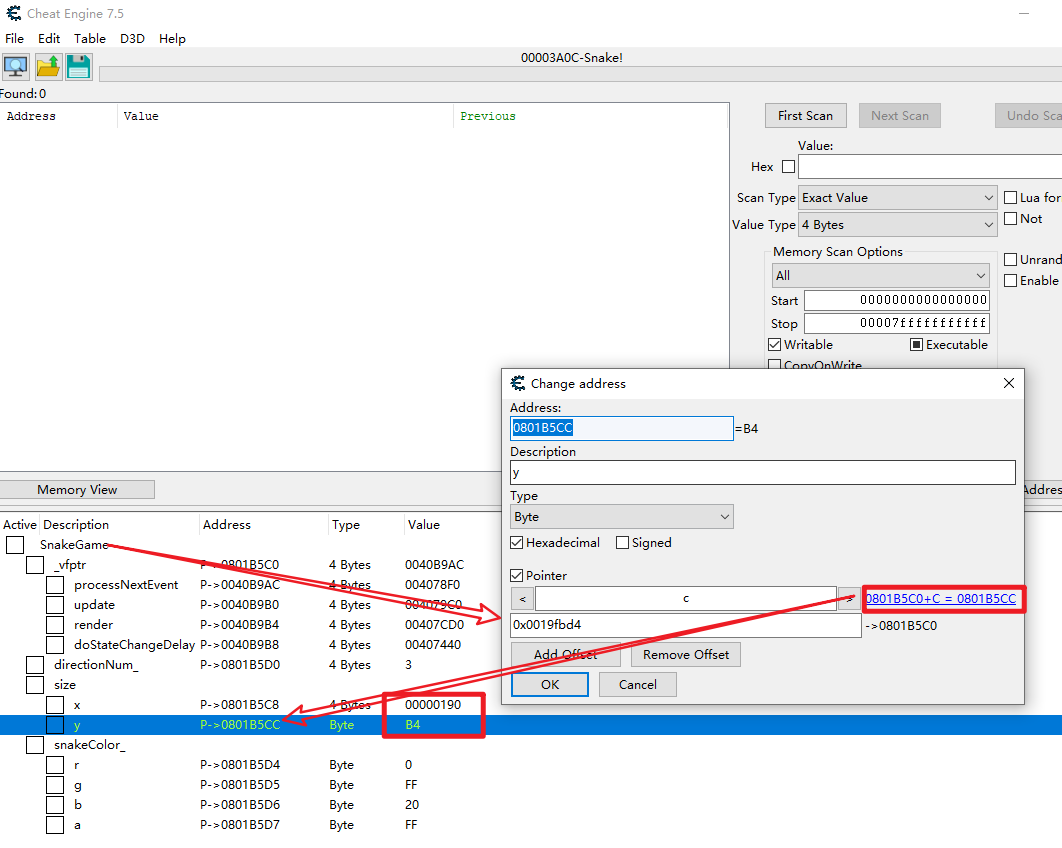
\includegraphics[width=0.85\linewidth]{CE_MEM_TREE.png}
        \caption{层级内存}
        \label{fig:CE_MEM_TREE}
    \end{figure}
\end{frame}

\begin{frame}[fragile]
    \LogoFrametitle{CE 监视内存}
    \normalsize
    \textbf{总结:} \\
    \begin{enumerate}
        \item 通过平坦式内存全局观察所有的内存单元变化.比如SnakeGame的内存偏移就说明是线性存储了数据.
        \item 通过对象字段存储的地址继续进一步观察,不断得到下一级数据,从而得到纵向的存储数据.
    \end{enumerate}
    纵横内存分析,即可描绘出完整的嵌套式数据结构.
    \linespread{1} \selectfont
\end{frame}


\subsection{SnakeGame 内存分析this的成员含义}
\begin{frame}[fragile]
    \LogoFrametitle{对象内存分析}
    \href{URL}{时间旅行反汇编AddrFlowEasy.asm} \\

    \scriptsize
    \begin{table}[htbp] % 自动找最合适的位置放置该表格
        \centering % 整个表格居中
        \caption{SnakeGame Object Memory Parse}
        \begin{tabular}{p{1cm}p{5cm}}
            \toprule
            \multicolumn{2}{l}{\textbf{Class members by offset base on memory line}} \\
            行  65: & ;[edx+0x4]=[0x08A66894]=0x08A66890                              \\
            行  68: & ;[edx+0x8]=[0x08A66898]=0x00000190                              \\
            行  71: & ;[edx+0xC]=[0x08A6689C]=0x00000150                              \\
            行  88: & ;[edx]=[0x08A66890]=0x00406708                                  \\
            行  93: & ;[edx+0x10]=[0x08A668A0]=0x00000003                             \\
            行 141: & ;[esi+0x24]=[0x08A668B4]=0x41200000                             \\
            行 212: & ;[eax]=[0x08A668C0]=0x004066E8                                  \\
            行 230: & ;[ecx+0x4]=[0x08A668C4]=0x07836E98                              \\
            行 237: & ;[ecx+0xC]=[0x08A668CC]=0x00000003                              \\
            行 242: & ;[ecx+0x10]=[0x08A668D0]=0x41700000                             \\
            行 245: & ;[ecx+0x14]=[0x08A668D4]=0x41800000                             \\
            行 251: & ;[eax]=[0x08A668D8]=0xFF94FF00                                  \\
            行 356: & ;[ecx+0x8]=[0x08A668C8]=0x00000001                              \\
            行 469: & ;[esi]=[0x08A67C80]=0x08A36778                                  \\
        \end{tabular}
    \end{table}
\end{frame}

\begin{frame}[fragile]{对象内存分析}
    \tiny
    \linespread{0.5} \selectfont
    \begin{x86asmcode}
        /*0x00403691*/    mov edx, ecx
        /*0x00403693*/    mov dword ptr ss:[ebp-0x20], edx
        ;[ebp-0x20]=[0x0019FBF8]=0x00000001
        ;[ebp-0x20]=[0x0019FBF8]=0x08A66890  <-- Modify
    \end{x86asmcode}
    通过ecx推断可知0x08A66890是Object对象的首地址.根据上面的表格的地址计算0x08A66890的偏移,并结合赋值推测变量的类型和含义。
    \tiny
    \begin{table}[htbp] % 自动找最合适的位置放置该表格
        \centering % 整个表格居中
        \caption{SnakeGame Object Memory Parse}
        \begin{tabular}{p{1cm}p{5cm}p{4cm}}
            \toprule
            \multicolumn{3}{l}{\textbf{Class members by offset base on memory line}} \\
            行  65: & ;[edx+0x4]=[0x08A66894]=0x08A66890  & +Offset 0x4               \\[0.6ex]
            行  68: & ;[edx+0x8]=[0x08A66898]=0x00000190  & +Offset 0x8               \\[0.6ex]
            行  71: & ;[edx+0xC]=[0x08A6689C]=0x00000150  & +Offset 0xc               \\[0.6ex]
            行  88: & ;[edx]=[0x08A66890]=0x00406708      & +Offset 0x0               \\[0.6ex]
            行  93: & ;[edx+0x10]=[0x08A668A0]=0x00000003 & +Offset 0x10              \\[0.6ex]
            行 141: & ;[esi+0x24]=[0x08A668B4]=0x41200000 & +Offset 0x24              \\[0.6ex]
            行 212: & ;[eax]=[0x08A668C0]=0x004066E8      & +Offset 0x30              \\[0.6ex]
            行 230: & ;[ecx+0x4]=[0x08A668C4]=0x07836E98  & +Offset 0x34              \\[0.6ex]
            行 237: & ;[ecx+0xC]=[0x08A668CC]=0x00000003  & +Offset 0x3c              \\[0.6ex]
            行 242: & ;[ecx+0x10]=[0x08A668D0]=0x41700000 & +Offset 0x40              \\[0.6ex]
            行 245: & ;[ecx+0x14]=[0x08A668D4]=0x41800000 & +Offset 0x44              \\[0.6ex]
            行 251: & ;[eax]=[0x08A668D8]=0xFF94FF00      & +Offset 0x48              \\[0.6ex]
            行 356: & ;[ecx+0x8]=[0x08A668C8]=0x00000001  & +Offset 0x38              \\[0.6ex]
            行 469: & ;[esi]=[0x08A67C80]=0x08A36778      & +Offset 0x13f0            \\[0.6ex]
        \end{tabular}
    \end{table}
\end{frame}
\begin{frame}[fragile]{对象内存分析}
    \tiny
    \begin{table}[htbp] % 自动找最合适的位置放置该表格
        \centering % 整个表格居中
        \caption{SnakeGame Object Memory Parse}
        \begin{tabular}{p{1cm}p{5cm}p{4cm}}
            \toprule
            \multicolumn{3}{l}{\textbf{Class members by offset base on memory line}} \\
            行  65: & ;[edx+0x4]=[0x08A66894]=0x08A66890  & 猜测系统DLL的函数                \\[0.6ex]
            行  68: & ;[edx+0x8]=[0x08A66898]=0x00000190  & SizeX                     \\[0.6ex]
            行  71: & ;[edx+0xC]=[0x08A6689C]=0x00000150  & SizeY                     \\[0.6ex]
            行  88: & ;[edx]=[0x08A66890]=0x00406708      & 猜测本模块的函数地址,虚表?            \\[0.6ex]
            行  93: & ;[edx+0x10]=[0x08A668A0]=0x00000003 & 枚举值                       \\[0.6ex]
            行 141: & ;[esi+0x24]=[0x08A668B4]=0x41200000 & 浮点数                       \\[0.6ex]
            行 212: & ;[eax]=[0x08A668C0]=0x004066E8      & 猜测本模块的函数地址,虚表?            \\[0.6ex]
            行 230: & ;[ecx+0x4]=[0x08A668C4]=0x07836E98  & 猜测系统DLL的函数                \\[0.6ex]
            行 237: & ;[ecx+0xC]=[0x08A668CC]=0x00000003  & 枚举值                       \\[0.6ex]
            行 242: & ;[ecx+0x10]=[0x08A668D0]=0x41700000 & 浮点数:15.0                  \\[0.6ex]
            行 245: & ;[ecx+0x14]=[0x08A668D4]=0x41800000 & 浮点数:16.0                  \\[0.6ex]
            行 251: & ;[eax]=[0x08A668D8]=0xFF94FF00      & ???                       \\[0.6ex]
            行 356: & ;[ecx+0x8]=[0x08A668C8]=0x00000001  & 枚举值或者bool值                \\[0.6ex]
            行 469: & ;[esi]=[0x08A67C80]=0x08A36778      & 猜测系统DLL的函数                \\[0.6ex]
        \end{tabular}
    \end{table}
\end{frame}
%%%%%%%%%%%%%%%%%%%%%%%%%%%%%%%%%%%%%%%%%%%%%%%%%%%%%%%%%%%%%


%---------------------------------------------------------------------------------------

\section{SnakeGameApp}
\subsection{SnakeGameApp::updateCurrentState}

\begin{frame}[fragile]
    \LogoFrametitle{虚函数简单识别}
    \begin{x86asmcode}
        0040906B  mov   edx,dword ptr [eax+4]
        0040906E  call  edx\end{x86asmcode}
    0040906E call调用目标是寄存器,说明edx存放的是函数指针,从0040906B处edx通过eax+4解引用得到的。初步确认edx存放的是虚函数指针,而eax是虚表的首地址.eax进一步在内存中确认:\\
    0x0040B9AC  f0 78 40 00  \\
    0x0040B9B0  c0 79 40 00  \\
    0x0040B9B4  d0 7c 40 00  \\
    0x0040B9B8  40 74 40 00  \\
    0x0040B9BC  60 78 40 00  \\
    从上面的存放内容,基本就可以确认是虚表内容了.如果某个对象存放了这个eax,那么那个引用地址就是虚表的所属的对象了。
\end{frame}

\begin{frame}[fragile]{虚函数简单识别}
    \textbf{总结:} \\ call 后面的寄存器是由一个地址加偏移的结果解引用得到的,那么就大胆的猜测它就是虚函数吧!
\end{frame}



\end{document}
